\chapter{Compound word inflection}

\label{chap-multiflex}
MULTIFLEX is a multi-lingual Unicode-compatible platform for automatic inflection of 
\textit{multi-word units} (MWUs), also known as \textit{compound words}. It is
\index{Multi-word units}\index{MWU}\index{Compound words}
meant in particular for the creation of morphological dictionaries of MWUs. 
It implements a unification-based formalism (\cite{Savary05}) 
for the description of inflectional behavior of MWUs which supposes the
existence of a module for the inflectional morphology of simple words.
 
\bigskip
\noindent In this chapter, we present the notion of multi-word unit and we
describe the method to inflect them with MULTIFLEX. 

\bigskip
\noindent This chapter is derived from the MULTIFLEX manual, written by Agata
Savary, the author of MULTIFLEX.

%%%%%%%%%%%%%%%%%%%%%%%%%%%%%%%%%%%%%%%%%%%%%%%%%%%%%%%%%%%%%
\section{Multi-Word Units}
\label{section:MWUs}
Multi-word units (MWUs) encompass a bunch of hard-to-define and controversial 
linguistic objects (cf. \cite{HabertJacquemin93}, \cite{Corbin92}). Their numerous 
linguistic and pragmatic definitions (\cite{Benven74}, \cite{Downing77}, \cite{Levi78}, 
\cite{Bauer83}, \cite{Gross90}, \cite{Anscombre90}, \cite{max-1993},
\cite{Gross96}, \cite{Cadiot92}) invoke three major points:

\begin{itemize}
\item they are composed of two or more words
\item they show some degree of morphological, distributional or semantic non-compositionality
\item they have unique and constant references 
\end{itemize}

\bigskip
\noindent However, the basic notions (a word, a reference, the
non-compositionality) and measures (degree of non-compositionality), used 
in those definitions are themselves controversial.

\bigskip
\noindent Pragmatically, we consider a MWU as a 
contiguous sequence of \textit{graphical units} \index{Graphical units}which,
for some application-dependent reasons, has to be listed, described 
(morphologically, syntactically, semantically, etc.) 
and processed as a unit.

\subsection{Formal Description of the Inflectional Behavior of Multi-word Units}
\label{subsec:MWUs inflection}
The main issue in MULTIFLEX is the inflectional morphology of MWUs. This phenomenon has 
been linguistically analyzed for English, Polish and French in \cite{these-Savary}. 

\bigskip
\noindent Obviously, a reliable inflection processing of single words is a
necessary condition for the inflection processing of MWUs. However, this condition 
is rarely a sufficient one. For example, in order to obtain the plural form of 

\begin{itemize}
\item \emph{battle cry}
\item \emph{battle royal}
\item \emph{battle of nerves}
\end{itemize}

\noindent in English, not only do we need to know how to generate the plural 
of \emph{battle, royal} and \emph{cry}, but also to know how different
inflected forms of these constituents combine:

\begin{itemize}
\item \emph{battle cr\underline{ies}}
\item \emph{battle royal\underline{s}}, or \emph{battle\underline{s} royal},
\item \emph{battle\underline{s} of nerves}
\end{itemize}

\noindent but not
 
\begin{itemize}
\item[*] {\emph{battle\underline{s} cr\underline{ies}}}
\item[*] {\emph{battle\underline{s} royal\underline{s}}}
\item[*] {\emph{battle\underline{s} of nerve\underline{ }}}
\end{itemize}

\bigskip
\noindent Formally, a fully explicit description of the inflectional paradigms of 
MWUs requires an answer to the following questions:

\begin{itemize}
\item What is the MWU's morphological class (noun, adjective, etc.) and thus what 
inflection categories (number, gender, case, etc.) are relevant to it? \cite{PrzepWol03} 
argue for a morphosyntactically motivated definition of morphological classes: a morphological 
class should fully determine the inflection categories the word inflects for as well as those 
that are lexically fixed for the word, e.g. in Polish, a noun has a gender and inflects for number and case.
\item What are the exceptions to the inflection categories determined above? E.g. in Polish 

\begin{itemize}
\item \emph{wybory powszechne}\\
 (\emph{general election}) 
\end{itemize}

is a compound noun but it doesn't have a singular form (although its head word \emph{wybory} does).
\item What are the inflectional characteristics (base form, morphological class, inflection 
paradigm, etc.) of the single constituents of the MWU? E.g. in French, \emph{porte} (\emph{door}) 
is an uninflected verb in 

\begin{itemize}
\item \emph{porte-avion} \\
 (\emph{aircraft carrier}) 
\end{itemize}

while it is an inflected noun in
 
\begin{itemize}
\item \emph{porte-fen\^etre} \\
(\emph{French window}) 
\end{itemize}

which takes an \emph{s} in plural 

\begin{itemize}
\item \emph{porte\underline{s}-fen\^etre\underline{s}}
\end{itemize} 
\item How should we combine the inflected forms of the single constituents in order to generate the inflected forms of the whole compound? E.g. to inflect \emph{battle of nerves} and \emph{battle cry} in number we need to inflect the first and the last constituent, respectively. 
\end{itemize}

%%%%%%%%%%%%%%%%%%%%%%%%%%%%%%%%%%%%%%%%%%%%%%%%%%%%%%%%%%%%%
\subsection{Lexicalized vs. Grammar-Based Approach to Morphological Description}
A previous study (\cite{these-Savary}) has confirmed the status of MWUs
as units on the frontier between morphology and syntax. Their compound structure suggests 
productivity which can hardly be processed without a grammar-based approach.
However some of their morphological, syntactic and semantic properties exclude their 
processing merely in terms of the properties of their constituents. For example, 
in both examples below:

\begin{itemize}
\item \emph{chief justice}
\item \emph{lord justice}
\end{itemize} 

\noindent there are few automatically accessible hints indicating that the former one is morphologically 
a standard English \emph{Noun Noun} phrase taking an \emph{s} at its last constituent in plural, 
while the plural of the latter has three variants:
 
\begin{itemize}
\item \emph{chief justice\underline{s}}
\item \emph{lord justice\underline{s}, lord\underline{s} justice,
lord\underline{s} justice\underline{s}}
\end{itemize}
 
\bigskip
\noindent Thus, at least one of the above examples has to be considered as lexicalized in 
order for the automatic morphological processing to be reliable.

\bigskip
\noindent MULTIFLEX implements a unification-based formalism for the
description of the inflectional behavior of MWUs presented in \cite{Savary05}. Its features are described 
in section~\ref{section:formalism}. This formalism requires the description to
be \emph{fully} lexicalized: each MWU listed in a dictionary obtains a code (e.g. \emph{NC\_NN, NC\_NN2}, etc.) 
representing its inflectional paradigm, for instance, in the DELA-like format:
\[
\begin{array}[c]{l}
  $aircraft carrier(carrier.N1:s),\textbf{NC\_NN}$ \\
  $chief justice(justice.N1:s),\textbf{NC\_NN}$ \\
  $lord(lord.N1:s) justice(justice.N1:s),\textbf{NC\_NN2}$ \\
  \dots
\end{array}
\]

\bigskip
\noindent However, only a few codes, which can be seen as a phrase grammar of the 
language, represent the big majority of all MWUs. Thus, the lexicalization of the 
description mainly consists of pointing out the MWUs which respect or don't respect 
the ``grammar''.

%%%%%%%%%%%%%%%%%%%%%%%%%%%%%%%%%%%%%%%%%%%%%%%%%%%%%%%%%%%%%
\section{Formalism for the Computational Morphology of MWUs}
\label{section:formalism}
In \cite{Savary05} was proposed a formalism for describing the morphological 
paradigms of MWUs. It has been based on studies of English, Polish and French, and 
further tested for Serbian \cite{Krstevetal06}. It consists of a language-independent 
kernel which is to be completed by a set of morphological elements characteristic for the 
given language. In this section we give an in-depth description of this
formalism.

%%%%%%%%%%%%%%%%%%%%%%%%%%%%%%%%%%%%%%%%%%%%%%%%%%%%%%%%%%%%%
\subsection{Morphological Features of the Language}
\label{subsec:langfeat}
When processing MWUs of a given language we have to provide some general data about 
that language. These data are included in two textual files.

\index{\verb+Morphology.txt+}\index{File!\verb+Morphology.txt+}\bigskip
\noindent The \verb+Morphology.txt+ file gives the morphological classes 
(noun, adjective,\dots), categories (number, gender, case,\dots) and values 
(masculine, feminine, singular, nominative,\dots). Consider the following example:
\[
\begin{array}[c]{ll}
$Polish$ \\
$$<$CATEGORIES$>$$ \\
$Nb: sing, pl$ \\
$Case: Nom, Gen, Dat, Acc, Inst, Loc, Voc$ \\
$Gen: masc\_pers, masc\_anim, masc\_inanim, fem, neu$ \\
$$<$CLASSES$>$)$ \\
$noun: (Nb,$<$var$>$),(Case,$<$var$>$),(Gen,$<$fixed$>$)$ \\
$adj:(Nb,$<$var$>$),(Case,$<$var$>$),(Gen,$<$var$>$)$ \\
$adv:$
\end{array}
\]

\bigskip
\noindent The above file says that, for Polish, three inflection categories are 
considered: the number (\emph{Nb}), the case (\emph{Case}) and the gender (\emph{Gen}). 
Each category is given an exhaustive list of its possible values (singular and plural 
for number, etc.). Further, each morphological class is described with respect to the 
categories it inflects for, and those that are fixed for it. For example, a noun inflects 
for  number and case, and has a (fixed) gender. The presence of such a file is necessary 
if we wish to express the fact that a certain word inflects for number, gender or case, 
without having to explicitly enumerate each time which inflectional values (singular, 
plural, masculine, etc.) it can take.

\index{\verb+Morphology.txt+}\index{File!\verb+Morphology.txt+}
\bigskip
\noindent Similarly, for French the \verb+Morphology.txt+ file may be as
follows:
\[
\begin{array}[c]{l}
$French$ \\
$$<$CATEGORIES$>$$ \\
$Nb: s, p$ \\
$Gen: m, f$ \\
$$<$CLASSES$>$$\\
$noun: (Nb,$<$var$>$),(Gen,$<$var$>$)$ \\
$adj:(Nb,$<$var$>$),(Gen,$<$var$>$)$ \\
$adv:$
\end{array}
\]

\bigskip
\noindent However, in the existing systems for computational morphology, such a
description of classes, categories and values is not always present. For example, according to the DELA 
conventions (\cite{dicos-francais}) the morphological values of each simple word are plain 
sequences of characters (e.g. \emph{ms} for masculine singular) without any explicit mention 
of their corresponding categories. In order for the program to be compatible
with such systems, we use a list (contained in a file
called\index{\verb+Equivalences.txt+}\index{File!\verb+Equivalences.txt+}
\verb+Equivalences.txt+) that describes which foreign inflectional feature
corresponds to which category-value pair in our description. For example, the following lists:
\[
\begin{array}[c]{ll}
Polish                        &French\\
s: Nb=sing                    &s: Nb=s  \\
p: Nb=pl                      &p: Nb=p \\
M: Case=Nom                   &f: Gen=f  \\
D: Case=Gen                   &m: Gen=m    \\
C: Case=Dat  &\\
B: Case=Acc  &\\
I: Case=Inst  &\\
L: Case=Loc  &\\
V: Case=Voc  &\\
o: Gen=masc\_pers  &\\
z: Gen=masc\_anim  &\\
r: Gen=masc\_inanim  &\\
f: Gen=fem  &\\
n: Gen=neu &
\end{array}
\]

\bigskip
\noindent describe the equivalences between the previous \verb+Morphology.txt+
file for Polish and French, respectively, and the single-character features that might be used in 
DELA dictionaries for those languages under Unitex.

%%%%%%%%%%%%%%%%%%%%%%%%%%%%%%%%%%%%%%%%%%%%%%%%%%%%%%%%%%%%%
\subsection{Decomposition of a MWU into Units}
\label{subsec:decomp}
The notion of an elementary graphical unit is controversial and varies across languages 
and NLP systems. For instance in nitex an alphabet, i.e. a set of characters, is
first defined for each language. Each non alphabet character is called a separator. A graphical 
unit is then either a single separator (usually a punctuation mark, a digit, etc.) or a 
contiguous sequence of alphabet characters (e.g. \emph{aujourd'hui} in French consists, 
according to this definition, of 3 units). In other systems a graphical unit may contain 
a punctuation mark (e.g. \emph{c'est-\`a-dire}), or a limit between two graphical units 
may occur within a sequence of alphabet characters (\emph{widzia\l $\mid$bym}, cf \cite{PrzepWol03}). 

\bigskip
\noindent This variety of possible definitions of a graphical unit obviously has an 
impact on the definition of a multi-word unit. However, we wish our formalism for MWUs 
to be adaptable to different morphological systems for ``simple words''. Thus, the 
definition of a graphical unit is a parameter to our system: each time MULTIFLEX is 
used with an external module for single units, this module has to decide how a sequence 
of characters is to be divided into units.

\bigskip
\noindent In our formalism, units are referred to by numerical variables \emph{\$1, \$2, \$3}, etc. 
For example with Unitex, a sequence like

\begin{itemize}
\item \emph{Athens '04}
\end{itemize} 

\bigskip
\noindent consists of five constituents referred to in MULTIFLEX as:
\[
\begin{array}[c]{l}
$\$1 = \emph{Athens}$ \\
$\$2 = $<$space$>$$ \\
$\$3 = \emph{'}$ \\
$\$4 = \emph{0}$ \\
$\$5 = \emph{4}$ \\
\end{array}
\]

\bigskip
\noindent Each simple unit subject to inflection within a MWU has to be morphologically 
identified. The identification means providing sufficient data so that any inflected form 
of the same item may be generated on demand. For instance in:
\begin{itemize}
\item \emph{m\'emoire vive}
\end{itemize} 
we need to know that \emph{vive} is the feminine singular form of a lemma, and we have to 
be able to generate the feminine plural form of the same lemma, \emph{vives}. We suppose 
that the external module for single units working with MULTIFLEX is responsible for such 
identification and generation of inflected forms of single units.

\bigskip
\noindent In Unitex, the generation of forms is strongly inspired by the DELA
system (\cite{dicos-francais}). In order to be able to generate one or more 
inflected forms of a word we have to know:

\begin{itemize}
\item its lemma
\item its inflection paradigm (called inflection code)
\item the inflection features of forms to be generated
\end{itemize}

\bigskip
\noindent Thus, within the Unitex/MULTIFLEX interface the description of a
single unit is done as follows:

\begin{itemize}
\item \emph{vive(vif.A54:fs)}
\end{itemize} 

\bigskip
\noindent where \emph{A54} is the inflection code of \emph{vif} and \emph{fs} is the DELA-style 
description using morphological features appearing in \verb+Equivalences.txt+
file (cf section~\ref{subsec:langfeat}). Knowing that \emph{vive} is a feminine
singular form of \emph{vif} we may demand the generation of its plural without having to 
explicitly indicate the plural of which gender we are interested in: since we only wish to 
change the number, the gender remains as in the original word \emph{vive}, i.e. feminine.

\subsection{Inflection paradigm of a MWU}
\label{subsec:paradigm}
The morphological description of MWUs in our formalism is inspired by the DELA system in the sense that:

\begin{itemize}
\item each MWU is attributed an inflection code
\item a MWU's inflection code explicitly describes each inflected form of a MWU in terms 
of actions to be performed on the lemma, and inflectional features to be attached to each form  
\end{itemize}

\bigskip
\noindent In the Unitex-interfaced version, MULTIFLEX uses inflection codes
represented as Unitex graphs compiled into the \verb+.fst2+ format. For example,
Figure~\ref{fig:BattleRoyal} contains the inflection graph for \emph{battle royal}.

\begin{figure}[!htb]
  \centering
  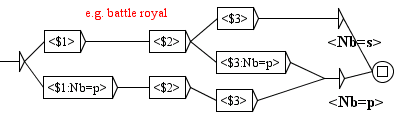
\includegraphics[width=10cm]{resources/img/BattleRoyal.png}
  \caption{Inflection graph for \emph{battle royal}}
  \label{fig:BattleRoyal}
\end{figure}

\bigskip
\noindent According to the Unitex convention, three constituents are present 
in \emph{battle royal}: \emph{battle} referred to as \emph{\$1}, a space referred 
to as \emph{\$2}, and \emph{royal} referred to as \emph{\$3}. If a variable appears 
alone in a box the constituent has to be the same as in the lemma of the MWU. For 
instance, $<$\$3$>$ in the uppermost path means that the unit \emph{royal} is to be 
recopied as such. If the variable is accompanied by a set of category-feature equations, 
the constituent has to be inflected to the required form. E.g.  $<$\$3:Nb=p$>$ means that 
the plural form of \emph{royal} is needed. 

\bigskip
\noindent In order to generate all inflected forms of the MWU we have to explore all 
the paths existing in the graph. Each path starts at the leftmost right arrow and ends 
at the final encircled box. Each time we come to a node we perform the action contained 
in the box (a recopy or an inflection of a constituent) and we accumulate the morphological 
features contained under the box. The total of the accumulated node outputs should result in 
the complete morphological description of the inflected form.

\bigskip
\noindent For example in the graph on Figure~\ref{fig:BattleRoyal} if we
follow the intermediate path shown on Figure~\ref{fig:BattleRoyalonepath}:

\begin{figure}[!htb]
  \centering
  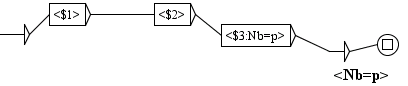
\includegraphics[width=10cm]{resources/img/BattleRoyalonepath.png}
  \caption{One path of the inflection graph for \emph{battle royal}}
  \label{fig:BattleRoyalonepath}
\end{figure}

\bigskip
\noindent we recopy \emph{battle} (\emph{\$1}) and the space (\emph{\$2}), and we put \emph{royal} 
into plural, which yields the plural form  \emph{battle royals} of the whole MWU. As the graph 
on Figure~\ref{fig:BattleRoyal} contains three different paths the whole set of inflected forms 
generated for \emph{battle royal} would be: 
\[
\begin{array}[l]{l}
\emph{battle royal $<$Nb=s$>$} \\
\emph{battle royals $<$Nb=p$>$} \\
\emph{battles royal $<$Nb=p$>$}
\end{array}
\]
\bigskip
\noindent After rewriting these forms into the Unitex DELACF format we obtain
the following entries:
\[
\begin{array}[l]{l}
\emph{battle royal,battle royal.N:s} \\
\emph{battle royals,battle royal.N:p} \\
\emph{battles royal,battle royal.N:p}
\end{array}
\]

\bigskip
\noindent Note that this description is independent of the way we generate inflected forms 
of single words because we suppose that this problem is handled by an existing external 
morphological system for single words. In the Unitex-interfaced version of
MULTIFLEX, we would generate the plural of \emph{royal} due to the fact that its lemma is known as having 
the inflection code \emph{N1} represented on Figure \ref{fig:N1}.

\begin{figure}[!htb]
  \centering
  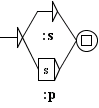
\includegraphics[width=2.8cm]{resources/img/N1'EN.png}
  \caption{Inflection graph \emph{N1} for simple words inflecting like \emph{royal}}
  \label{fig:N1}
\end{figure}

\bigskip
\noindent In an inflection paradigm of a MWU, each constituent is accompanied only by those 
morphological categories which it should inflect for. The categories that remain unchanged 
don't have to be mentioned. For instance, in \emph{bateau-mouche} in French (a Paris-style 
river-boat), both noun constituents have their gender set but they inflect in 
number: \emph{bateau\underline{x}-mouche\underline{s}}. That's why on Figure~\ref{fig:BateauMouche1} 
containing the inflection graph for this MWU, the corresponding boxes contain value assignments for 
number only. Note that both constituents may or may not agree in gender, here \emph{bateau} 
is masculine while \emph{mouche} is feminine.

\begin{figure}[!htb]
  \centering
  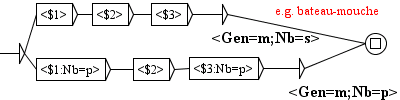
\includegraphics[width=10cm]{resources/img/BateauMouche1.png}
  \caption{Inflection graph for MWUs inflection like \emph{bateau-mouche}}
  \label{fig:BateauMouche1}
\end{figure}

%%%%%%%%%%%%%%%%%%%%%%%%%%%%%%%%%%%%%%%%%%%%%%%%%%%%%%%%%%%%%
\subsubsection{Unification Variables}
An important feature of our formalism are \textit{unification variables}.
\index{Unification variables}They are introduced by the dollar sign followed by
an identifier which may contain any number of characters, e.g. \emph{\$g1}, \emph{\$num\_10}, \emph{\$c}, etc.
For example, Figure~\ref{fig:BateauMouche2} shows a graph roughly 
equivalent\footnote{Up to the case when single constituents appearing in the lemma 
of a MWU are already in plural, as in \emph{cross-road\underline{s}}.} to the one 
on Figure~\ref{fig:BateauMouche1} in the sense that it allows to generate the same 
inflected forms for the same MWUs. However, this time a single path represents both 
the singular and the plural form. That is possible due to the unification variable 
\emph{\$n} which may be instantiated to any value of the domain of its category (\emph{Nb}), 
here \emph{\$n=s} or \emph{\$n=p}. The instantiation is unique for all elements on a path: 
if we fix the singular value for the first constituent the same value has to be set for the 
third one, as well as for the whole MWU. Similarly, if we fix \emph{\$n} to \emph{p} while 
processing the first node it has to remain \emph{p} until the end of the path.

\begin{figure}[!htb]
  \centering
  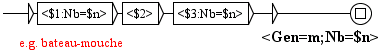
\includegraphics[width=10cm]{resources/img/BateauMouche2.png}
  \caption{Inflection graph for \emph{bateau-mouche} with a unification variable}
  \label{fig:BateauMouche2}
\end{figure}

\bigskip
\noindent The inflection graph on Figure~\ref{fig:BateauMouche2} applies to most kinds of 
French compounds of types \emph{Noun Noun} and \emph{Noun Adjective} (\emph{bateau-mouche, 
ange gardien, circuit s\'equentiel}, etc.) which are of masculine gender. That is 
because the output of the final node contains \emph{Gen=m}. For all compounds of the same 
types but of feminine gender, e.g. \emph{main courante, moissoneuse-batteuse}, etc., a new 
graph has to be created which is identical to Figure~\ref{fig:BateauMouche2} up to the final 
output containing \emph{$<$Gen=f;Nb=\$n$>$}. That is not very intuitive since 
\emph{circuit s\'equentiel} and \emph{main courante} inflect in the same way, in the sense 
that in both cases we need to put the first and the last constituent to plural in order to 
obtain the plural form of the whole MWU. 

\bigskip
\noindent That's why another type of instantiation for unification variables has been introduced. 
It is accompanied by a double equal sign (\emph{==}) (as opposed to the 
single equal sign \emph{=} as for \emph{\$n} on Figure~\ref{fig:BateauMouche2}). 
If a unification variable is assigned to a category by this symbol then it
inherits the value of this category from the corresponding constituent, as it appears in the lemma of 
the MWU. For instance, Figure~\ref{fig:BateauMouche3} contains a graph describing the inflected 
forms for both masculine and feminine French compounds of types \emph{Noun Noun} and 
\emph{Noun Adjective}. Its first box contains the double assignment of the gender to variable 
\emph{\$g} which means that this variable has its value fixed to the gender value of the first 
constituent. For \emph{bateau-mouche} it is fixed to masculine because \emph{bateau} is 
masculine while for \emph{main courante} it is fixed to feminine. 

\begin{figure}[!htb]
  \centering
  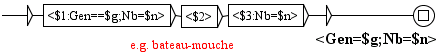
\includegraphics[width=11cm]{resources/img/BateauMouche3.png}
  \caption{Inflection graph for \emph{bateau-mouche} with two types of instantiation}
  \label{fig:BateauMouche3}
\end{figure}

\bigskip
\noindent Note that the double assignment, contrary to the single assignment, no longer means 
that the variable is to be instantiated to all values of the corresponding category domain. It 
has a unique value all through the path on which it appears, even if it is concerned by another, 
single, assignment somewhere else on the same path. For example, on Figure~\ref{fig:BateauMouche3} 
the final output contains \emph{Gen=\$g} but \emph{\$g} may only take one value determined by the 
first constituent.

\bigskip
\noindent Unification variables are particularly useful in highly inflected languages. For 
example, in Polish most nouns inflect for number (2 values) and case (7 values), which implies 
at least 14 different forms (if variants and syncretic forms are distinguished). This score is 
even higher for adjectives which inflect for number, case and gender (3 till 9 values, according 
to different approaches). If no unification mechanism were available each of these numerous 
forms would have to be described by a separate path in the graph. The use of unification variables 
allows to dramatically reduce the size of the graph (to one path only in most cases). 

\bigskip
\noindent For example, Figure~\ref{fig:PranieMozgu} shows the graph for Polish compounds that 
inflect like \emph{pranie m\'ozgu} (\emph{brainwashing}) or \emph{powo\.zenie koniem} 
(\emph{horse coaching}). Their third constituent has its case fixed (most often to genitive or 
instrumental). Their first and third constituent inflect in number independently from each other 
(\emph{pranie m\'ozg\underline{\'ow}}, \emph{prani\underline{a} m\'ozgu}, 
\emph{prani\underline{a} m\'ozg\underline{\'ow}}, etc.). That's why either of them has a different 
unification variable for number inflection (\emph{\$n1} and \emph{\$n2}). The three 
variables $\$n1$, $\$n2$, and $\$c$ may be instantiated to any value from their respective 
domains (\emph{\{sing,pl\}, \{sing,pl\}}, and \emph{\{Nom,Gen,Dat,Acc,Inst,Loc,Voc\}}; 
cf \verb+Morphology.txt+ file in section~\ref{subsec:langfeat}). The whole MWU
inherits its gender, number and case from its first constituent. Its gender is 
fixed (\emph{Gen==\$g}) while its number 
and case are instantiated to any of the 14 possible combinations. The single path in this graph 
would have to be replaced by 28 different ones if the use of unification variables were not allowed.

\begin{figure}[!htb]
  \centering
  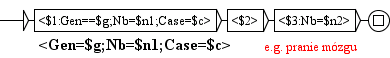
\includegraphics[width=10cm]{resources/img/PranieMozgu.png}
  \caption{Inflection graph for \emph{pranie m\'ozgu}}
  \label{fig:PranieMozgu}
\end{figure}


%%%%%%%%%%%%%%%%%%%%%%%%%%%%%%%%%%%%%%%%%%%%%%%%%%%%%%%%%%%%%
\subsubsection{Orthographic and Other Variants}
Our formalism allows for any constituent to be omitted or moved within different inflected 
forms if there is a need for that. It also enables the insertion of extra graphical units 
which do not appear in the base form of the MWU. This allows to extend an inflection paradigm 
to a more general variation description, e.g. orthographic or, partly, syntactic variation 
(see \cite{Jacquemin01} for an extensive study on term variation). For example, in English, 
\emph{student union} appears in corpus also as \emph{student\underline{s} union}, and 
\emph{student\underline{s'} union}, in singular or plural in each case. Our formalism 
allows to include both types of variation in one description (cf. Figure~\ref{fig:StudentUnion}).

\begin{figure}[!htb]
  \centering
  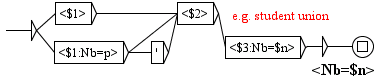
\includegraphics[width=10cm]{resources/img/StudentUnion.png}
  \caption{Inflection graph for \emph{student union}}
  \label{fig:StudentUnion}
\end{figure}

\bigskip
\noindent Figure~\ref{fig:BirthDate} shows an example in which, additionally to the insertion 
of a new constituent, the order of constituents may be reverted. The upper path allows to 
generate e.g. \emph{birth date} and  \emph{birth dates} while the lower one represents the 
syntactic variants of the previous forms: \emph{date of birth} and \emph{dates of birth}.

\begin{figure}[!htb]
  \centering
  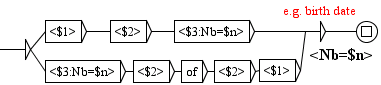
\includegraphics[width=10cm]{resources/img/BirthDate.png}
  \caption{Inflection graph for \emph{birth date}}
  \label{fig:BirthDate}
\end{figure}

%%%%%%%%%%%%%%%%%%%%%%%%%%%%%%%%%%%%%%%%%%%%%%%%%%%%%%%%%%%%%
\subsubsection{Interface with the Morphological System for Simple Words}
\label{Interface}
MULTIFLEX is an implementation of the formalism for the inflectional morphology of MWUs 
presented above. It supposes the existence of a morphological system for single words 
which satisfies the following interface constraints:

\begin{itemize}
\item For a given sequence of characters it returns its segmentation into indivisible graphical 
units (tokens) (cf section~\ref{subsec:decomp}). For instance, in case of
Unitex' definition of a token, sequence \emph{Athens '04} is to be divided into
5 tokens:
\[
\begin{array}[l]{l}
\emph{``Athens '04'' $\rightarrow$ (``Athens'','' ``,''''',''0'',''4'')}
\end{array}
\]

\item For a given simple inflected form it returns all its possible morphological 
identifications. A morphological identification has to allow the generation of any 
other inflected form of the same lemma on demand by the same morphological module. 
For instance, in case of Unitex, the form \emph{porte} yields 7 morphological 
identifications (6 of which are factorized with respect to their inflection code):
\[
\begin{array}[l]{l}
\emph{porte $\rightarrow$ ((porte,porte.N21:s),(porte,porter.V3:P1s:P3s:S1s:S3s:Y2s))}
\end{array}
\]

In case of ambigu\"\i ty, as above, the proper identification has to be done, for the time being, 
by the user during the edition of the MWU lemma to be inflected (in future, this task will be 
partly automated). For instance, in case of \emph{porte-fen\^etre} the first constituent has 
to be identified by the user as a noun rather than a verb.

\item For a given morphological identification and a set of inflectional values it returns 
all corresponding inflected forms. For instance, in Polish, if the instrumental forms of the 
word \emph{r\k{e}ka} are to be produced, three forms should be returned: \emph{r\k{e}k\k{a}} 
(singular instrumental), \emph{r\k{e}kami} and  \emph{r\k{e}koma} (two variants of the plural 
instrumental).
\[
\begin{array}[l]{lll}
\emph{(r\k{e}ka,$<$Case=Inst$>$)}&  \rightarrow    & \emph{((r\k{e}k\k{a},<Nb=sing;Gen=fem;Case=Inst>)}, \\
                                    &              & \emph{(r\k{e}kami,<Nb=pl;Gen=fem;Case=Inst>)}, \\
                                    &              & \emph{(r\k{e}koma,<Nb=pl;Gen=fem;Case=Inst>))}
\end{array}
\]
\end{itemize}

\bigskip
\noindent Such definition of an interface between the morphological system for simple words and 
the one for MWUs allows a better modularity and independence of one another. The latter doesn't 
need to know how inflected forms of simple words are described, analyzed and generated. It only 
requires a set of correct inflected forms of a MWU's constituents. Conversely, the former system 
knows nothing about how the latter one combines the provided forms to produce multi-word sequences.        
 
%%%%%%%%%%%%%%%%%%%%%%%%%%%%%%%%%%%%%%%%%%%%%%%%%%%%%%%%%%%%%
\section{Integration in Unitex}
\label{section:UNITEXinterface}
One of the major design principles of MULTIFLEX is to be as independent as possible of the 
morphological system for simple words. However, the existence of such a system is inevitable 
because MWUs consist of simple words which we need to be able to inflect in order to inflect 
a MWU as a whole.

\bigskip
\noindent In its present version, MULTIFLEX relies on the Unitex simple
word inflection system:

\begin{itemize}
\item MULTIFLEX uses the same character encoding standards as Unitex, i.e. Unicode 3.0.
\item MULTIFLEX uses the Unitex' graph editor for the representation of inflectional paradigms of MWUs.
\item MULTIFLEX admits similar principles of the morphological description as those admitted in 
the DELA system implemented in Unitex. Thus, an inflection paradigm is a set 
of actions to be performed on the lemma in order to generate its inflected forms, and of 
corresponding inflection features to be attached to each generated form.
\item MULTIFLEX allows to extend the Unitex dictionary treatment to the inflection of a DELAC 
(DELA electronic dictionary of compounds) into a DELACF (DELA electronic dictionary of 
compounds' inflected forms). The format of the generated DELACF is compatible with Unitex, 
while the format of the DELAC is novel but inspired from the one of the DELAS (DELA electronic 
dictionary of simple words).
\end{itemize}

\bigskip
\noindent The following sections present, for several languages, complete examples of a DELAC into DELACF 
inflection within the MULTIFLEX/Unitex interface.

%%%%%%%%%%%%%%%%%%%%%%%%%%%%%%%%%%%%%%%%%%%%%%%%%%%%%%%%%%%%%
\subsection{Complete Example in English}
Let us assume that the description of morphological features of English is given
by the following \verb+Morphology.txt+ file:
\[
\begin{array}[l]{l}
$English$ \\
$<CATEGORIES>$ \\
$Nb:s,p$ \\
$<CLASSES>$ \\
$noun:(Nb,<var>)$ \\
$adj:$
\end{array}
\]

\bigskip
\noindent and that the equivalences between these features and their corresponding codes in DELA dictionaries 
are given by the following \verb+Equivalences.txt+ file: 
\[
\begin{array}[l]{l}
$English$ \\
$s : Nb=s$ \\
$p : Nb=p$ \\
\end{array}
\]

\bigskip
\noindent Consider the following sample English DELAC file:

\begin{verbatim}
angle(angle.N1:s) of reflection,NC_NXXXX
Adam's apple(apple.N1:s),NC_XXXXN
air brake(brake.N1:s),NC_XXN
birth date(date.N1:s),NC_NN_NofN
criminal police,NC_XXXinv
cross-roads,NC_XXNs
head(head.N1:s) of government(government.N1:s),NC_NofNs
notary(notary.N3:s) public(public.N1:s),NC_NsNs
rolling stone(stone.N1:s),NC_XXN
student(student.N1:s) union(union.N1:s),NC_Ns'N
\end{verbatim}

\bigskip
\noindent The corresponding inflection graphs \emph{N1} and \emph{N3} for simple words are 
represented on figures~\ref{fig:N1'EN} and ~\ref{fig:N3'EN} while those for compounds are shown 
on figures~\ref{fig:NC'NXXXX'EN} through~\ref{fig:NC'Ns'N'EN}. 

\bigskip
\noindent The DELACF dictionary resulting from the inflection, via MULTIFLEX, of the above DELAC 
is as follows:

\begin{verbatim}
angle of reflection,angle of reflection.NC_NXXXX:s
angles of reflection,angle of reflection.NC_NXXXX:p
Adam's apple,Adam's apple.NC_XXXXN:s
Adam's apples,Adam's apple.NC_XXXXN:p
air brake,air brake.NC_XXN:s
air brakes,air brake.NC_XXN:p
date of birth,birth date.NC_NN_NofN:s
dates of birth,birth date.NC_NN_NofN:p
birth date,birth date.NC_NN_NofN:s
birth dates,birth date.NC_NN_NofN:p
criminal police,criminal police.NC_XXXinv:p
cross-roads,cross-roads.NC_XXNs:s
cross-roads,cross-roads.NC_XXNs:p
heads of government,head of government.NC_NofNs:p
heads of governments,head of government.NC_NofNs:p
head of government,head of government.NC_NofNs:s
notaries public,notary public.NC_NsNs:p
notary public,notary public.NC_NsNs:s
notary publics,notary public.NC_NsNs:p
rolling stone,rolling stone.NC_XXN:s
rolling stones,rolling stone.NC_XXN:p
students' union,student union.NC_Ns'N:s
students' unions,student union.NC_Ns'N:p
students union,student union.NC_Ns'N:s
students unions,student union.NC_Ns'N:p
student union,student union.NC_Ns'N:s
student unions,student union.NC_Ns'N:p
\end{verbatim}
 
\begin{figure}[ht]
\begin{minipage}[c]{0.45\textwidth}
 \centering
 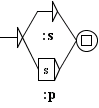
\includegraphics[width=2.5cm]{resources/img/N1'EN.png}
  \caption{Inflection graph \emph{N1} for English simple words}
  \label{fig:N1'EN}
\end{minipage}\hfill
\begin{minipage}[c]{0.5\textwidth}
 \centering
 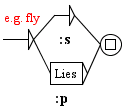
\includegraphics[width=3cm]{resources/img/N3'EN.png}
  \caption{Inflection graph \emph{N3} for English simple words}
  \label{fig:N3'EN}
\end{minipage}
\end{figure}

%%%%%%%%%%%%MWUs

\begin{figure}[!htb]
  \centering
  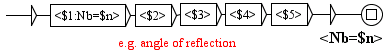
\includegraphics[width=10cm]{resources/img/NC'NXXXX'EN.png}
  \caption{Inflection graph \emph{NC\_NXXXX} for English MWUs}
  \label{fig:NC'NXXXX'EN}
\end{figure}

\begin{figure}[!htb]
  \centering
  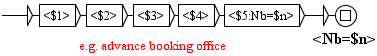
\includegraphics[width=9.7cm]{resources/img/NC'XXXXN'EN.png}
  \caption{Inflection graph \emph{NC\_XXXXN} for English MWUs}
  \label{fig:NC'XXXXN'EN}
\end{figure}

\begin{figure}[!htb]
  \centering
  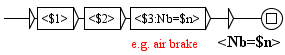
\includegraphics[width=7.8cm]{resources/img/NC'XXN'EN.png}
  \caption{Inflection graph \emph{NC\_XXN} for English MWUs}
  \label{fig:NC'XXN}
\end{figure}

\begin{figure}[!htb]
  \centering
  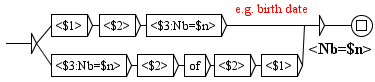
\includegraphics[width=10cm]{resources/img/NC'NN'NofN'EN.png}
  \caption{Inflection graph \emph{NC\_NN\_NofN} for English MWUs}
  \label{fig:NC'NN'NofN'EN}
\end{figure}

\begin{figure}[!htb]
  \centering
  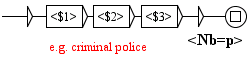
\includegraphics[width=7cm]{resources/img/NC'XXXinv'EN.png}
  \caption{Inflection graph \emph{NC\_XXXinv} for English MWUs}
  \label{fig:NC'XXXinv'EN}
\end{figure}

\begin{figure}[!htb]
  \centering
  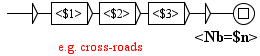
\includegraphics[width=7cm]{resources/img/NC'XXNs'EN.png}
  \caption{Inflection graph \emph{NC\_XXNs} for English MWUs}
  \label{fig:NC'XXNs'EN}
\end{figure}

\begin{figure}[!htb]
  \centering
  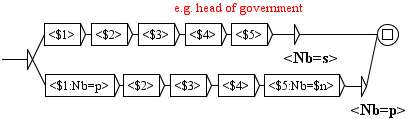
\includegraphics[width=10.4cm]{resources/img/NC'NofNs'EN.png}
  \caption{Inflection graph \emph{NC\_NofNs} for English MWUs}
  \label{fig:NC'NofNs'EN}
\end{figure}

\begin{figure}[!htb]
  \centering
  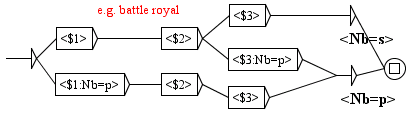
\includegraphics[width=10.4cm]{resources/img/NC'NsNs'EN.png}
  \caption{Inflection graph \emph{NC\_NsNs} for English MWUs}
  \label{fig:NC'NsNs'EN}
\end{figure}

\begin{figure}[!htb]
  \centering
  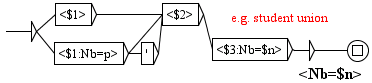
\includegraphics[width=9.8cm]{resources/img/NC'Ns'N'EN.png}
  \caption{Inflection graph \emph{NC\_Ns'N} for English MWUs}
  \label{fig:NC'Ns'N'EN}
\end{figure}

%%%%%%%%%%%%%%%%%%%%%%%%%%%%%%%%%%%%%%%%%%%%%%%%%%%%%%%%%%%%%
\subsection{Complete Example in French}
Let us assume that the description of morphological features of French is given
by the following \verb+Morphology.txt+ file:
\[
\begin{array}[l]{l}
$French$ \\
$<CATEGORIES>$ \\
$Nb : s, p$ \\
$Gen : m, f$ \\
$<CLASSES>$ \\
$noun : (Nb,<var>),(Gen,<var>)$ \\
$adj:(Nb,<var>),(Gen,<var>)$ \\
$adv:$
\end{array}
\]

\bigskip
\noindent and that the equivalences between these features and their corresponding codes 
in DELA dictionaries are given by the following \verb+Equivalences.txt+ file: 
\[
\begin{array}[l]{l}
$French$ \\
$s : Nb=s$ \\
$p : Nb=p$ \\
$m : Gen=m$ \\
$f : Gen=f$
\end{array}
\]

\bigskip
\noindent Consider the following sample French DELAC file (the DELAS inflection codes may 
vary from those present in UNITEX):

\begin{verbatim}
avant-garde(garde.N21:fs),NC_XXN
bateau(bateau.N3:ms)-mouche(mouche.N21:fs),NC_NN
caf�(caf�.N1:ms) au lait,NC_NXXXX
carte(carte.N21:fs) postale(postal.A8:fs),NC_NN$
cousin(cousin.N8:ms) germain(germain.A8:ms),NC_NNmf
franc(franc.A47:ms) ma�on(ma�on.N41:ms),NC_AN1
m�moire(m�moire.N21:fs) vive(vif.A48:fs),NC_NN
microscope(microscope.N1:ms) � effet tunnel,NC_NXXXXXX
porte-serviette(serviette.N21:fs),NC_VNm
\end{verbatim}


\bigskip
\noindent The corresponding inflection graphs for MWUs are shown on figures~\ref{fig:NC'XXN'FR} 
through~\ref{fig:NC'VNm'FR}. 

\bigskip
\noindent The DELACF dictionary resulting from the inflection, via MULTIFLEX, of the above 
DELAC is as follows:

\begin{verbatim}
avant-garde,avant-garde.NC_XXN:fs
avant-gardes,avant-garde.NC_XXN:fp
bateau-mouche,bateau-mouche.NC_NN:ms
bateaux-mouches,bateau-mouche.NC_NN:mp
caf� au lait,caf� au lait.NC_NXXXX:ms
caf�s au lait,caf� au lait.NC_NXXXX:mp
carte postale,carte postale.NC_NN:fs
cartes postales,carte postale.NC_NN:fp
cousin germain,cousin germain.NC_NNmf:ms
cousins germains,cousin germain.NC_NNmf:mp
cousine germaine,cousin germain.NC_NNmf:fs
cousines germaines,cousin germain.NC_NNmf:fp
franc-ma�on,franc ma�on.NC_AN1:ms
franc-ma�onne,franc ma�on.NC_AN1:fs
franc ma�on,franc ma�on.NC_AN1:ms
franc ma�onne,franc ma�on.NC_AN1:fs
francs-ma�ons,franc ma�on.NC_AN1:mp
francs-ma�onnes,franc ma�on.NC_AN1:fp
francs ma�ons,franc ma�on.NC_AN1:mp
francs ma�onnes,franc ma�on.NC_AN1:fp
m�moire vive,m�moire vive.NC_NN:fs
m�moires vives,m�moire vive.NC_NN:fp
microscope � effet tunnel,microscope � effet tunnel.NC_NXXXXXX:ms
microscopes � effet tunnel,microscope � effet tunnel.NC_NXXXXXX:mp
porte-serviette,porte-serviette.NC_VNm:ms
porte-serviettes,porte-serviette.NC_VNm:ms
porte-serviettes,porte-serviette.NC_VNm:mp 
\end{verbatim}


\begin{figure}[!htb]
  \centering
  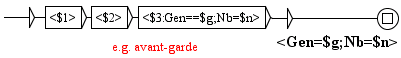
\includegraphics[width=10.2cm]{resources/img/NC'XXN'FR.png}
  \caption{Inflection graph \emph{NC\_XXN} for French MWUs}
  \label{fig:NC'XXN'FR}
\end{figure}

\begin{figure}[!htb]
  \centering
  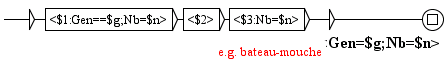
\includegraphics[width=10.8cm]{resources/img/NC'NN'FR.png}
  \caption{Inflection graph \emph{NC\_NN} for French MWUs}
  \label{fig:NC'NN'FR}
\end{figure}

\begin{figure}[!htb]
  \centering
  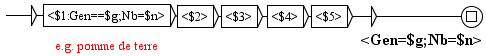
\includegraphics[width=12cm]{resources/img/NC'NXXXX'FR.png}
  \caption{Inflection graph \emph{NC\_NXXXX} for French MWUs}
  \label{fig:NC'NXXXX'FR}
\end{figure}

\begin{figure}[!htb]
  \centering
  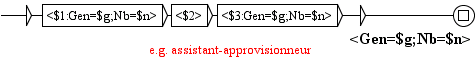
\includegraphics[width=12cm]{resources/img/NC'NNmf'FR.png}
  \caption{Inflection graph \emph{NC\_NNmf} for French MWUs}
  \label{fig:NC'NNmf'FR}
\end{figure}

\begin{figure}[!htb]
  \centering
  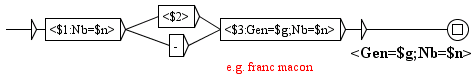
\includegraphics[width=12cm]{resources/img/NC'AN1'FR.png}
  \caption{Inflection graph \emph{NC\_AN1} for French MWUs}
  \label{fig:NC'AN1'FR}
\end{figure}

\begin{figure}[!htb]
  \centering
  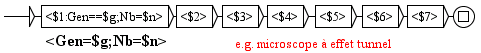
\includegraphics[width=12.2cm]{resources/img/NC'NXXXXXX'FR.png}
  \caption{Inflection graph \emph{NC\_NXXXXXX} for French MWUs}
  \label{fig:NC'NXXXXXX'FR}
\end{figure}

\begin{figure}[!htb]
  \centering
  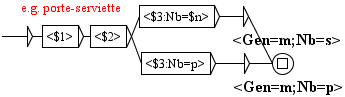
\includegraphics[width=9.2cm]{resources/img/NC'VNm'FR.png}
  \caption{Inflection graph \emph{NC\_VNm} for French MWUs}
  \label{fig:NC'VNm'FR}
\end{figure}


%%%%%%%%%%%%%%%%%%%%%%%%%%%%%%%%%%%%%%%%%%%%%%%%%%%%%%%%%%%%%
\subsection{Complete Example in Serbian}
Let us assume that the description of morphological features of Serbian is
given by the following \verb+Morphology.txt+ file:
\[
\begin{array}[l]{l}
$Serbian$ \\
$<CATEGORIES>$ \\
$Nb:s,p,w$ \\
$Case:1,2,3,4,5,6,7$ \\
$Gen:m,f,n$ \\
$Anim:v,q,g$ \\
$Comp:a,b,c$ \\
$Det:d,k,e$ \\
$<CLASSES>$ \\
$noun:(Nb,<var>),(Case,<var>),(Gen,<var>),(Anim,<fixed>)$ \\
$adj:(Nb,<var>),(Case,<var>),(Gen,<var>),(Anim,<var>),(Comp,<var>),(Det,<var>)$ \\
$adv:$
\end{array}
\]

\bigskip
\noindent The particuliarity of this morphological model is not only its reachness but also 
the existence of \emph{no-care} features like \emph{Anim=g} or \emph{Det=e}. These features 
agree with all other features in the same category. They are used only for some particular 
sublasses of nouns or adjectives and are necessary for a better compactness of the inflection 
paradigms of simple words which are already considerably huge, and would be even larger if 
no \emph{no-care} symbols were used.  

\bigskip
\noindent Let us assume that the equivalences between the above features and
their corresponding codes in DELA dictionaries are given by the following 
\verb+Equivalences.txt+ file:
\[
\begin{array}[l]{l}
$Serbian$ \\
$s:Nb=s$ \\
$p:Nb=p$ \\
$w:Nb=w$ \\
$1:Case=1$ \\
$2:Case=2$ \\
$3:Case=3$ \\
$4:Case=4$ \\
$5:Case=5$ \\
$6:Case=6$ \\
$7:Case=7$ \\
$m:Gen=m$ \\
$f:Gen=f$ \\
$n:Gen=n$ \\
$v:Anim=v$ \\
$q:Anim=q$ \\
$g:Anim=g$ \\
$a:Comp=a$ \\
$b:Comp=b$ \\
$c:Comp=c$ \\
$d:Det=d$ \\
$k:Det=k$ \\
$e:Det=e$
\end{array}
\]

\bigskip
\noindent Consider the following sample Serbian DELAC file (the DELAS inflection codes may 
vary from those present in Unitex):

\scriptsize
\begin{verbatim}
zxiro racyun(racyun.N1:ms1q),NC_2XN1+N+Comp
avio-prevoznik(prevoznik.N10:ms1v),NC_2XN2+N+Comp
predsednik(predsednik.N10:ms1v) drzxave(drzxava.N600:fs2q),NC_N2X1+N+Comp
Ujedinxene(Ujedinxen.A1:aefp1g) nacije(nacija.N600:fp1q),NC_AXN3+N+Comp+NProp+Org
Kosovo(Kosovo.N308:ns1q) i Metohija(Metohija.N623:fs1q),NC_N3XN+N+Comp+NProp+Top+Reg 
istrazxni(istrazxni.A2:adms1g) sudija(sudija.N679:ms1v),NC_AXNF+N+Comp
Mirosinka(Mirosinka.N1637:fs1v) Dinkicx(Dinkicx.N1028:ms1v),NC_ImePrezime+N+Comp+Hum+PersName
gladan(gladan.A18:akms1g) kao vuk(vuk.N128:ms1v),AC_A3XN2/hungry as a wolf
\end{verbatim}
\normalsize

\bigskip
\noindent The corresponding inflection graphs for MWUs are shown on
figures~\ref{fig:NC'2XN1'SRB}  through~\ref{fig:AC'A3XN2'SRB}. 

\bigskip
\noindent The DELACF dictionary resulting from the inflection, via MULTIFLEX, of the above DELAC is as follows:

\footnotesize
\begin{verbatim}
zxiro-racyun,zxiro racyun.NC_2XN1+N+Comp:s1qm
zxiro-racyuna,zxiro racyun.NC_2XN1+N+Comp:s2qm
zxiro-racyunu,zxiro racyun.NC_2XN1+N+Comp:s3qm
zxiro-racyun,zxiro racyun.NC_2XN1+N+Comp:s4qm
zxiro-racyune,zxiro racyun.NC_2XN1+N+Comp:s5qm
zxiro-racyunom,zxiro racyun.NC_2XN1+N+Comp:s6qm
zxiro-racyunu,zxiro racyun.NC_2XN1+N+Comp:s7qm
zxiro-racyuni,zxiro racyun.NC_2XN1+N+Comp:p1qm
zxiro-racyuna,zxiro racyun.NC_2XN1+N+Comp:p2qm
zxiro-racyunima,zxiro racyun.NC_2XN1+N+Comp:p3qm
zxiro-racyune,zxiro racyun.NC_2XN1+N+Comp:p4qm
zxiro-racyuni,zxiro racyun.NC_2XN1+N+Comp:p5qm
zxiro-racyunima,zxiro racyun.NC_2XN1+N+Comp:p6qm
zxiro-racyunima,zxiro racyun.NC_2XN1+N+Comp:p7qm
zxiro-racyuna,zxiro racyun.NC_2XN1+N+Comp:w2qm
zxiro-racyuna,zxiro racyun.NC_2XN1+N+Comp:w4qm
zxiro racyun,zxiro racyun.NC_2XN1+N+Comp:s1qm
zxiro racyuna,zxiro racyun.NC_2XN1+N+Comp:s2qm
zxiro racyunu,zxiro racyun.NC_2XN1+N+Comp:s3qm
zxiro racyun,zxiro racyun.NC_2XN1+N+Comp:s4qm
zxiro racyune,zxiro racyun.NC_2XN1+N+Comp:s5qm
zxiro racyunom,zxiro racyun.NC_2XN1+N+Comp:s6qm
zxiro racyunu,zxiro racyun.NC_2XN1+N+Comp:s7qm
zxiro racyuni,zxiro racyun.NC_2XN1+N+Comp:p1qm
zxiro racyuna,zxiro racyun.NC_2XN1+N+Comp:p2qm
zxiro racyunima,zxiro racyun.NC_2XN1+N+Comp:p3qm
zxiro racyune,zxiro racyun.NC_2XN1+N+Comp:p4qm
zxiro racyuni,zxiro racyun.NC_2XN1+N+Comp:p5qm
zxiro racyunima,zxiro racyun.NC_2XN1+N+Comp:p6qm
zxiro racyunima,zxiro racyun.NC_2XN1+N+Comp:p7qm
zxiro racyuna,zxiro racyun.NC_2XN1+N+Comp:w2qm
zxiro racyuna,zxiro racyun.NC_2XN1+N+Comp:w4qm
avio-prevoznik,avio-prevoznik.NC_2XN2+N+Comp:s1vm
avio-prevoznika,avio-prevoznik.NC_2XN2+N+Comp:s2vm
avio-prevozniku,avio-prevoznik.NC_2XN2+N+Comp:s3vm
avio-prevoznika,avio-prevoznik.NC_2XN2+N+Comp:s4vm
avio-prevoznicye,avio-prevoznik.NC_2XN2+N+Comp:s5vm
avio-prevoznikom,avio-prevoznik.NC_2XN2+N+Comp:s6vm
avio-prevozniku,avio-prevoznik.NC_2XN2+N+Comp:s7vm
avio-prevoznici,avio-prevoznik.NC_2XN2+N+Comp:p1vm
avio-prevoznika,avio-prevoznik.NC_2XN2+N+Comp:p2vm
avio-prevoznicima,avio-prevoznik.NC_2XN2+N+Comp:p3vm
avio-prevoznike,avio-prevoznik.NC_2XN2+N+Comp:p4vm
avio-prevoznici,avio-prevoznik.NC_2XN2+N+Comp:p5vm
avio-prevoznicima,avio-prevoznik.NC_2XN2+N+Comp:p6vm
avio-prevoznicima,avio-prevoznik.NC_2XN2+N+Comp:p7vm
avio-prevoznika,avio-prevoznik.NC_2XN2+N+Comp:w2vm
avio-prevoznika,avio-prevoznik.NC_2XN2+N+Comp:w4vm
avioprevoznik,avio-prevoznik.NC_2XN2+N+Comp:s1vm
avioprevoznika,avio-prevoznik.NC_2XN2+N+Comp:s2vm
avioprevozniku,avio-prevoznik.NC_2XN2+N+Comp:s3vm
avioprevoznika,avio-prevoznik.NC_2XN2+N+Comp:s4vm
avioprevoznicye,avio-prevoznik.NC_2XN2+N+Comp:s5vm
avioprevoznikom,avio-prevoznik.NC_2XN2+N+Comp:s6vm
avioprevozniku,avio-prevoznik.NC_2XN2+N+Comp:s7vm
avioprevoznici,avio-prevoznik.NC_2XN2+N+Comp:p1vm
avioprevoznika,avio-prevoznik.NC_2XN2+N+Comp:p2vm
avioprevoznicima,avio-prevoznik.NC_2XN2+N+Comp:p3vm
avioprevoznike,avio-prevoznik.NC_2XN2+N+Comp:p4vm
avioprevoznici,avio-prevoznik.NC_2XN2+N+Comp:p5vm
avioprevoznicima,avio-prevoznik.NC_2XN2+N+Comp:p6vm
avioprevoznicima,avio-prevoznik.NC_2XN2+N+Comp:p7vm
avioprevoznika,avio-prevoznik.NC_2XN2+N+Comp:w2vm
avioprevoznika,avio-prevoznik.NC_2XN2+N+Comp:w4vm
predsednik drzxave,predsednik drzxave.NC_N2X1+N+Comp:s1vm
predsednika drzxave,predsednik drzxave.NC_N2X1+N+Comp:s2vm
predsedniku drzxave,predsednik drzxave.NC_N2X1+N+Comp:s3vm
predsednika drzxave,predsednik drzxave.NC_N2X1+N+Comp:s4vm
predsednicye drzxave,predsednik drzxave.NC_N2X1+N+Comp:s5vm
predsednikom drzxave,predsednik drzxave.NC_N2X1+N+Comp:s6vm
predsedniku drzxave,predsednik drzxave.NC_N2X1+N+Comp:s7vm
predsednici drzxave,predsednik drzxave.NC_N2X1+N+Comp:p1vm
predsednici drzxava,predsednik drzxave.NC_N2X1+N+Comp:p1vm
predsednika drzxave,predsednik drzxave.NC_N2X1+N+Comp:p2vm
predsednika drzxava,predsednik drzxave.NC_N2X1+N+Comp:p2vm
predsednicima drzxave,predsednik drzxave.NC_N2X1+N+Comp:p3vm
predsednicima drzxava,predsednik drzxave.NC_N2X1+N+Comp:p3vm
predsednike drzxave,predsednik drzxave.NC_N2X1+N+Comp:p4vm
predsednike drzxava,predsednik drzxave.NC_N2X1+N+Comp:p4vm
predsednici drzxave,predsednik drzxave.NC_N2X1+N+Comp:p5vm
predsednici drzxava,predsednik drzxave.NC_N2X1+N+Comp:p5vm
predsednicima drzxave,predsednik drzxave.NC_N2X1+N+Comp:p6vm
predsednicima drzxava,predsednik drzxave.NC_N2X1+N+Comp:p6vm
predsednicima drzxave,predsednik drzxave.NC_N2X1+N+Comp:p7vm
predsednicima drzxava,predsednik drzxave.NC_N2X1+N+Comp:p7vm
predsednika drzxave,predsednik drzxave.NC_N2X1+N+Comp:w2vm
predsednika drzxava,predsednik drzxave.NC_N2X1+N+Comp:w2vm
predsednika drzxave,predsednik drzxave.NC_N2X1+N+Comp:w4vm
predsednika drzxava,predsednik drzxave.NC_N2X1+N+Comp:w4vm
Ujedinxene nacije,Ujedinxene nacije.NC_AXN3+N+Comp+NProp+Org:fp1q
Ujedinxenih nacija,Ujedinxene nacije.NC_AXN3+N+Comp+NProp+Org:fp2q
Ujedinxenima nacijama,Ujedinxene nacije.NC_AXN3+N+Comp+NProp+Org:fp3q
Ujedinxenim nacijama,Ujedinxene nacije.NC_AXN3+N+Comp+NProp+Org:fp3q
Ujedinxene nacije,Ujedinxene nacije.NC_AXN3+N+Comp+NProp+Org:fp4q
Ujedinxene nacije,Ujedinxene nacije.NC_AXN3+N+Comp+NProp+Org:fp5q
Ujedinxenima nacijama,Ujedinxene nacije.NC_AXN3+N+Comp+NProp+Org:fp6q
Ujedinxenim nacijama,Ujedinxene nacije.NC_AXN3+N+Comp+NProp+Org:fp6q
Ujedinxenima nacijama,Ujedinxene nacije.NC_AXN3+N+Comp+NProp+Org:fp7q
Ujedinxenim nacijama,Ujedinxene nacije.NC_AXN3+N+Comp+NProp+Org:fp7q
Kosovo i Metohija,Kosovo i Metohija.NC_N3XN+N+Comp+NProp+Top+Reg:ns1q
Kosova i Metohije,Kosovo i Metohija.NC_N3XN+N+Comp+NProp+Top+Reg:ns2q
Kosovu i Metohiji,Kosovo i Metohija.NC_N3XN+N+Comp+NProp+Top+Reg:ns3q
Kosovo i Metohiju,Kosovo i Metohija.NC_N3XN+N+Comp+NProp+Top+Reg:ns4q
Kosovo i Metohijo,Kosovo i Metohija.NC_N3XN+N+Comp+NProp+Top+Reg:ns5q
Kosovom i Metohijom,Kosovo i Metohija.NC_N3XN+N+Comp+NProp+Top+Reg:ns6q
Kosovu i Metohiji,Kosovo i Metohija.NC_N3XN+N+Comp+NProp+Top+Reg:ns7q
istrazxne sudije,istrazxni sudija.NC_AXNF+N+Comp:1vfp
istrazxnih sudija,istrazxni sudija.NC_AXNF+N+Comp:2vfp
istrazxnima sudijama,istrazxni sudija.NC_AXNF+N+Comp:3vfp
istrazxnim sudijama,istrazxni sudija.NC_AXNF+N+Comp:3vfp
istrazxne sudije,istrazxni sudija.NC_AXNF+N+Comp:4vfp
istrazxne sudije,istrazxni sudija.NC_AXNF+N+Comp:5vfp
istrazxnima sudijama,istrazxni sudija.NC_AXNF+N+Comp:6vfp
istrazxnim sudijama,istrazxni sudija.NC_AXNF+N+Comp:6vfp
istrazxnima sudijama,istrazxni sudija.NC_AXNF+N+Comp:7vfp
istrazxnim sudijama,istrazxni sudija.NC_AXNF+N+Comp:7vfp
istrazxne sudije,istrazxni sudija.NC_AXNF+N+Comp:2vfw
istrazxne sudije,istrazxni sudija.NC_AXNF+N+Comp:4vfw
istrazxnoga sudiju,istrazxni sudija.NC_AXNF+N+Comp:ms4v
istrazxnog sudiju,istrazxni sudija.NC_AXNF+N+Comp:ms4v
istrazxni sudija,istrazxni sudija.NC_AXNF+N+Comp:1vms
istrazxnoga sudije,istrazxni sudija.NC_AXNF+N+Comp:2vms
istrazxnog sudije,istrazxni sudija.NC_AXNF+N+Comp:2vms
istrazxnomu sudiji,istrazxni sudija.NC_AXNF+N+Comp:3vms
istrazxnome sudiji,istrazxni sudija.NC_AXNF+N+Comp:3vms
istrazxnom sudiji,istrazxni sudija.NC_AXNF+N+Comp:3vms
istrazxnomu sudiji,istrazxni sudija.NC_AXNF+N+Comp:7vms
istrazxnome sudiji,istrazxni sudija.NC_AXNF+N+Comp:7vms
istrazxnom sudiji,istrazxni sudija.NC_AXNF+N+Comp:7vms
istrazxni sudijo,istrazxni sudija.NC_AXNF+N+Comp:5vms
istrazxni sudija,istrazxni sudija.NC_AXNF+N+Comp:5vms
istrazxnim sudijom,istrazxni sudija.NC_AXNF+N+Comp:6vms
Dinkicx Mirosinka,Mirosinka Dinkicx.NC_ImePrezime+N+Comp+Hum+PersName:s1vf
Dinkicx Mirosinke,Mirosinka Dinkicx.NC_ImePrezime+N+Comp+Hum+PersName:s2vf
Dinkicx Mirosinki,Mirosinka Dinkicx.NC_ImePrezime+N+Comp+Hum+PersName:s3vf
Dinkicx Mirosinku,Mirosinka Dinkicx.NC_ImePrezime+N+Comp+Hum+PersName:s4vf
Dinkicx Mirosinka,Mirosinka Dinkicx.NC_ImePrezime+N+Comp+Hum+PersName:s5vf
Dinkicx Mirosinkom,Mirosinka Dinkicx.NC_ImePrezime+N+Comp+Hum+PersName:s6vf
Dinkicx Mirosinki,Mirosinka Dinkicx.NC_ImePrezime+N+Comp+Hum+PersName:s7vf
Mirosinka Dinkicx,Mirosinka Dinkicx.NC_ImePrezime+N+Comp+Hum+PersName:s1vf
Mirosinke Dinkicx,Mirosinka Dinkicx.NC_ImePrezime+N+Comp+Hum+PersName:s2vf
Mirosinki Dinkicx,Mirosinka Dinkicx.NC_ImePrezime+N+Comp+Hum+PersName:s3vf
Mirosinku Dinkicx,Mirosinka Dinkicx.NC_ImePrezime+N+Comp+Hum+PersName:s4vf
Mirosinka Dinkicx,Mirosinka Dinkicx.NC_ImePrezime+N+Comp+Hum+PersName:s5vf
Mirosinkom Dinkicx,Mirosinka Dinkicx.NC_ImePrezime+N+Comp+Hum+PersName:s6vf
Mirosinki Dinkicx,Mirosinka Dinkicx.NC_ImePrezime+N+Comp+Hum+PersName:s7vf
gladni kao vuk,gladan kao vuk.AC_A3XN2:s1mgda//hungry as a wolf
gladan kao vuk,gladan kao vuk.AC_A3XN2:s1mgka//hungry as a wolf
gladna kao vuk,gladan kao vuk.AC_A3XN2:s1fgea//hungry as a wolf
gladno kao vuk,gladan kao vuk.AC_A3XN2:s1ngea//hungry as a wolf
gladnoga kao vuk,gladan kao vuk.AC_A3XN2:s2mgda//hungry as a wolf
gladnog kao vuk,gladan kao vuk.AC_A3XN2:s2mgda//hungry as a wolf
gladna kao vuk,gladan kao vuk.AC_A3XN2:s2mgka//hungry as a wolf
gladne kao vuk,gladan kao vuk.AC_A3XN2:s2fgea//hungry as a wolf
gladnoga kao vuk,gladan kao vuk.AC_A3XN2:s2ngda//hungry as a wolf
gladnog kao vuk,gladan kao vuk.AC_A3XN2:s2ngda//hungry as a wolf
gladna kao vuk,gladan kao vuk.AC_A3XN2:s2ngka//hungry as a wolf
gladnome kao vuk,gladan kao vuk.AC_A3XN2:s3mgda//hungry as a wolf
gladnom kao vuk,gladan kao vuk.AC_A3XN2:s3mgda//hungry as a wolf
gladnu kao vuk,gladan kao vuk.AC_A3XN2:s3mgka//hungry as a wolf
gladnoj kao vuk,gladan kao vuk.AC_A3XN2:s3fgea//hungry as a wolf
gladnome kao vuk,gladan kao vuk.AC_A3XN2:s3ngda//hungry as a wolf
gladnom kao vuk,gladan kao vuk.AC_A3XN2:s3ngda//hungry as a wolf
gladnu kao vuk,gladan kao vuk.AC_A3XN2:s3ngka//hungry as a wolf
gladnu kao vuk,gladan kao vuk.AC_A3XN2:s4fgea//hungry as a wolf
gladno kao vuk,gladan kao vuk.AC_A3XN2:s4ngea//hungry as a wolf
gladni kao vuk,gladan kao vuk.AC_A3XN2:s5mgea//hungry as a wolf
gladna kao vuk,gladan kao vuk.AC_A3XN2:s5fgea//hungry as a wolf
gladno kao vuk,gladan kao vuk.AC_A3XN2:s5ngea//hungry as a wolf
gladnim kao vuk,gladan kao vuk.AC_A3XN2:s6mgea//hungry as a wolf
gladnom kao vuk,gladan kao vuk.AC_A3XN2:s6fgea//hungry as a wolf
gladnim kao vuk,gladan kao vuk.AC_A3XN2:s6ngea//hungry as a wolf
gladnome kao vuk,gladan kao vuk.AC_A3XN2:s7mgda//hungry as a wolf
gladnom kao vuk,gladan kao vuk.AC_A3XN2:s7mgda//hungry as a wolf
gladnu kao vuk,gladan kao vuk.AC_A3XN2:s7mgka//hungry as a wolf
gladnoj kao vuk,gladan kao vuk.AC_A3XN2:s7fgea//hungry as a wolf
gladnome kao vuk,gladan kao vuk.AC_A3XN2:s7ngda//hungry as a wolf
gladnom kao vuk,gladan kao vuk.AC_A3XN2:s7ngda//hungry as a wolf
gladnu kao vuk,gladan kao vuk.AC_A3XN2:s7ngka//hungry as a wolf
gladni kao vuk,gladan kao vuk.AC_A3XN2:p1mgea//hungry as a wolf
gladni kao vuci,gladan kao vuk.AC_A3XN2:p1mgea//hungry as a wolf
gladni kao vukovi,gladan kao vuk.AC_A3XN2:p1mgea//hungry as a wolf
gladne kao vuk,gladan kao vuk.AC_A3XN2:p1fgea//hungry as a wolf
gladne kao vuci,gladan kao vuk.AC_A3XN2:p1fgea//hungry as a wolf
gladne kao vukovi,gladan kao vuk.AC_A3XN2:p1fgea//hungry as a wolf
gladna kao vuk,gladan kao vuk.AC_A3XN2:p1ngea//hungry as a wolf
gladna kao vuci,gladan kao vuk.AC_A3XN2:p1ngea//hungry as a wolf
gladna kao vukovi,gladan kao vuk.AC_A3XN2:p1ngea//hungry as a wolf
gladnih kao vuk,gladan kao vuk.AC_A3XN2:p2mgea//hungry as a wolf
gladnih kao vuci,gladan kao vuk.AC_A3XN2:p2mgea//hungry as a wolf
gladnih kao vukovi,gladan kao vuk.AC_A3XN2:p2mgea//hungry as a wolf
gladnih kao vuk,gladan kao vuk.AC_A3XN2:p2fgea//hungry as a wolf
gladnih kao vuci,gladan kao vuk.AC_A3XN2:p2fgea//hungry as a wolf
gladnih kao vukovi,gladan kao vuk.AC_A3XN2:p2fgea//hungry as a wolf
gladnih kao vuk,gladan kao vuk.AC_A3XN2:p2ngea//hungry as a wolf
gladnih kao vuci,gladan kao vuk.AC_A3XN2:p2ngea//hungry as a wolf
gladnih kao vukovi,gladan kao vuk.AC_A3XN2:p2ngea//hungry as a wolf
gladnima kao vuk,gladan kao vuk.AC_A3XN2:p3mgea//hungry as a wolf
gladnima kao vuci,gladan kao vuk.AC_A3XN2:p3mgea//hungry as a wolf
gladnima kao vukovi,gladan kao vuk.AC_A3XN2:p3mgea//hungry as a wolf
gladnim kao vuk,gladan kao vuk.AC_A3XN2:p3mgea//hungry as a wolf
gladnim kao vuci,gladan kao vuk.AC_A3XN2:p3mgea//hungry as a wolf
gladnim kao vukovi,gladan kao vuk.AC_A3XN2:p3mgea//hungry as a wolf
gladnima kao vuk,gladan kao vuk.AC_A3XN2:p3fgea//hungry as a wolf
gladnima kao vuci,gladan kao vuk.AC_A3XN2:p3fgea//hungry as a wolf
gladnima kao vukovi,gladan kao vuk.AC_A3XN2:p3fgea//hungry as a wolf
gladnim kao vuk,gladan kao vuk.AC_A3XN2:p3fgea//hungry as a wolf
gladnim kao vuci,gladan kao vuk.AC_A3XN2:p3fgea//hungry as a wolf
gladnim kao vukovi,gladan kao vuk.AC_A3XN2:p3fgea//hungry as a wolf
gladnima kao vuk,gladan kao vuk.AC_A3XN2:p3ngea//hungry as a wolf 
gladnima kao vuci,gladan kao vuk.AC_A3XN2:p3ngea//hungry as a wolf
gladnima kao vukovi,gladan kao vuk.AC_A3XN2:p3ngea//hungry as a wolf
gladnim kao vuk,gladan kao vuk.AC_A3XN2:p3ngea//hungry as a wolf
gladnim kao vuci,gladan kao vuk.AC_A3XN2:p3ngea//hungry as a wolf
gladnim kao vukovi,gladan kao vuk.AC_A3XN2:p3ngea//hungry as a wolf
gladne kao vuk,gladan kao vuk.AC_A3XN2:p4mgea//hungry as a wolf
gladne kao vuci,gladan kao vuk.AC_A3XN2:p4mgea//hungry as a wolf
gladne kao vukovi,gladan kao vuk.AC_A3XN2:p4mgea//hungry as a wolf
gladne kao vuk,gladan kao vuk.AC_A3XN2:p4fgea//hungry as a wolf
gladne kao vuci,gladan kao vuk.AC_A3XN2:p4fgea//hungry as a wolf
gladne kao vukovi,gladan kao vuk.AC_A3XN2:p4fgea//hungry as a wolf
gladna kao vuk,gladan kao vuk.AC_A3XN2:p4ngea//hungry as a wolf
gladna kao vuci,gladan kao vuk.AC_A3XN2:p4ngea//hungry as a wolf
gladna kao vukovi,gladan kao vuk.AC_A3XN2:p4ngea//hungry as a wolf
gladni kao vuk,gladan kao vuk.AC_A3XN2:p5mgea//hungry as a wolf
gladni kao vuci,gladan kao vuk.AC_A3XN2:p5mgea//hungry as a wolf
gladni kao vukovi,gladan kao vuk.AC_A3XN2:p5mgea//hungry as a wolf
gladne kao vuk,gladan kao vuk.AC_A3XN2:p5fgea//hungry as a wolf
gladne kao vuci,gladan kao vuk.AC_A3XN2:p5fgea//hungry as a wolf
gladne kao vukovi,gladan kao vuk.AC_A3XN2:p5fgea//hungry as a wolf
gladna kao vuk,gladan kao vuk.AC_A3XN2:p5ngea//hungry as a wolf
gladna kao vuci,gladan kao vuk.AC_A3XN2:p5ngea//hungry as a wolf
gladna kao vukovi,gladan kao vuk.AC_A3XN2:p5ngea//hungry as a wolf
gladnima kao vuk,gladan kao vuk.AC_A3XN2:p6mgea//hungry as a wolf
gladnima kao vuci,gladan kao vuk.AC_A3XN2:p6mgea//hungry as a wolf
gladnima kao vukovi,gladan kao vuk.AC_A3XN2:p6mgea//hungry as a wolf
gladnim kao vuk,gladan kao vuk.AC_A3XN2:p6mgea//hungry as a wolf
gladnim kao vuci,gladan kao vuk.AC_A3XN2:p6mgea//hungry as a wolf
gladnim kao vukovi,gladan kao vuk.AC_A3XN2:p6mgea//hungry as a wolf
gladnima kao vuk,gladan kao vuk.AC_A3XN2:p6fgea//hungry as a wolf
gladnima kao vuci,gladan kao vuk.AC_A3XN2:p6fgea//hungry as a wolf
gladnima kao vukovi,gladan kao vuk.AC_A3XN2:p6fgea//hungry as a wolf
gladnim kao vuk,gladan kao vuk.AC_A3XN2:p6fgea//hungry as a wolf
gladnim kao vuci,gladan kao vuk.AC_A3XN2:p6fgea//hungry as a wolf
gladnim kao vukovi,gladan kao vuk.AC_A3XN2:p6fgea//hungry as a wolf
gladnima kao vuk,gladan kao vuk.AC_A3XN2:p6ngea//hungry as a wolf
gladnima kao vuci,gladan kao vuk.AC_A3XN2:p6ngea//hungry as a wolf
gladnima kao vukovi,gladan kao vuk.AC_A3XN2:p6ngea//hungry as a wolf
gladnim kao vuk,gladan kao vuk.AC_A3XN2:p6ngea//hungry as a wolf
gladnim kao vuci,gladan kao vuk.AC_A3XN2:p6ngea//hungry as a wolf
gladnim kao vukovi,gladan kao vuk.AC_A3XN2:p6ngea//hungry as a wolf
gladnima kao vuk,gladan kao vuk.AC_A3XN2:p7mgea//hungry as a wolf
gladnima kao vuci,gladan kao vuk.AC_A3XN2:p7mgea//hungry as a wolf
gladnima kao vukovi,gladan kao vuk.AC_A3XN2:p7mgea//hungry as a wolf
gladnim kao vuk,gladan kao vuk.AC_A3XN2:p7mgea//hungry as a wolf
gladnim kao vuci,gladan kao vuk.AC_A3XN2:p7mgea//hungry as a wolf
gladnim kao vukovi,gladan kao vuk.AC_A3XN2:p7mgea//hungry as a wolf
gladnima kao vuk,gladan kao vuk.AC_A3XN2:p7fgea//hungry as a wolf
gladnima kao vuci,gladan kao vuk.AC_A3XN2:p7fgea//hungry as a wolf
gladnima kao vukovi,gladan kao vuk.AC_A3XN2:p7fgea//hungry as a wolf
gladnim kao vuk,gladan kao vuk.AC_A3XN2:p7fgea//hungry as a wolf
gladnim kao vuci,gladan kao vuk.AC_A3XN2:p7fgea//hungry as a wolf
gladnim kao vukovi,gladan kao vuk.AC_A3XN2:p7fgea//hungry as a wolf
gladnima kao vuk,gladan kao vuk.AC_A3XN2:p7ngea//hungry as a wolf
gladnima kao vuci,gladan kao vuk.AC_A3XN2:p7ngea//hungry as a wolf
gladnima kao vukovi,gladan kao vuk.AC_A3XN2:p7ngea//hungry as a wolf
gladnim kao vuk,gladan kao vuk.AC_A3XN2:p7ngea//hungry as a wolf
gladnim kao vuci,gladan kao vuk.AC_A3XN2:p7ngea//hungry as a wolf
gladnim kao vukovi,gladan kao vuk.AC_A3XN2:p7ngea//hungry as a wolf
gladna kao vuk,gladan kao vuk.AC_A3XN2:w2mgea//hungry as a wolf
gladna kao vuci,gladan kao vuk.AC_A3XN2:w2mgea//hungry as a wolf
gladna kao vukovi,gladan kao vuk.AC_A3XN2:w2mgea//hungry as a wolf
gladne kao vuk,gladan kao vuk.AC_A3XN2:w2fgea//hungry as a wolf
gladne kao vuci,gladan kao vuk.AC_A3XN2:w2fgea//hungry as a wolf
gladne kao vukovi,gladan kao vuk.AC_A3XN2:w2fgea//hungry as a wolf
gladna kao vuk,gladan kao vuk.AC_A3XN2:w2ngea//hungry as a wolf
gladna kao vuci,gladan kao vuk.AC_A3XN2:w2ngea//hungry as a wolf
gladna kao vukovi,gladan kao vuk.AC_A3XN2:w2ngea//hungry as a wolf
gladna kao vuk,gladan kao vuk.AC_A3XN2:w4mgea//hungry as a wolf
gladna kao vuci,gladan kao vuk.AC_A3XN2:w4mgea//hungry as a wolf
gladna kao vukovi,gladan kao vuk.AC_A3XN2:w4mgea//hungry as a wolf
gladne kao vuk,gladan kao vuk.AC_A3XN2:w4fgea//hungry as a wolf
gladne kao vuci,gladan kao vuk.AC_A3XN2:w4fgea//hungry as a wolf
gladne kao vukovi,gladan kao vuk.AC_A3XN2:w4fgea//hungry as a wolf
gladna kao vuk,gladan kao vuk.AC_A3XN2:w4ngea//hungry as a wolf
gladna kao vuci,gladan kao vuk.AC_A3XN2:w4ngea//hungry as a wolf
gladna kao vukovi,gladan kao vuk.AC_A3XN2:w4ngea//hungry as a wolf
\end{verbatim}
\normalsize

\begin{figure}[!htb]
  \centering
  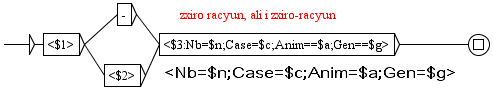
\includegraphics[width=12.4cm]{resources/img/NC'2XN1'SRB.png}
  \caption{Inflection graph \emph{NC\_2XN1} for Serbian MWUs}
  \label{fig:NC'2XN1'SRB}
\end{figure}

\begin{figure}[!htb]
  \centering
  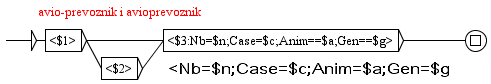
\includegraphics[width=12.4cm]{resources/img/NC'2XN2'SRB.png}
  \caption{Inflection graph \emph{NC\_2XN2} for Serbian MWUs}
  \label{fig:NC'2XN2'SRB}
\end{figure}

\begin{figure}[!htb]
  \centering
  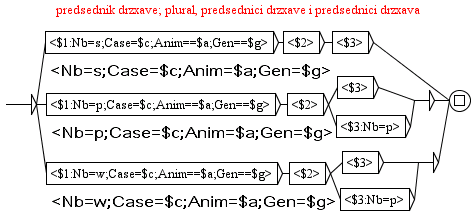
\includegraphics[width=12.2cm]{resources/img/NC'N2X1'SRB.png}
  \caption{Inflection graph \emph{NC\_N2X1} for Serbian MWUs}
  \label{fig:NC'N2X1'SRB}
\end{figure}

\begin{figure}[!htb]
  \centering
  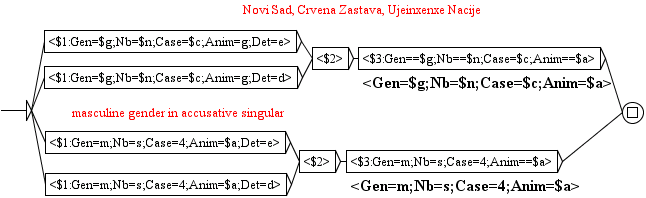
\includegraphics[width=15cm]{resources/img/NC'AXN3'SRB.png}
  \caption{Inflection graph \emph{NC\_AXN3} for Serbian MWUs}
  \label{fig:NC'AXN3'SRB}
\end{figure}

\begin{figure}[!htb]
  \centering
  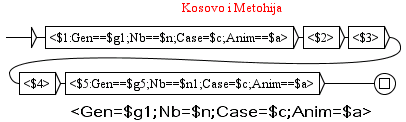
\includegraphics[width=10cm]{resources/img/NC'N3XN'SRB.png}
  \caption{Inflection graph \emph{NC\_N3XN} for Serbian MWUs}
  \label{fig:NC'N3XN'SRB}
\end{figure}

\begin{figure}[!htb]
  \centering
  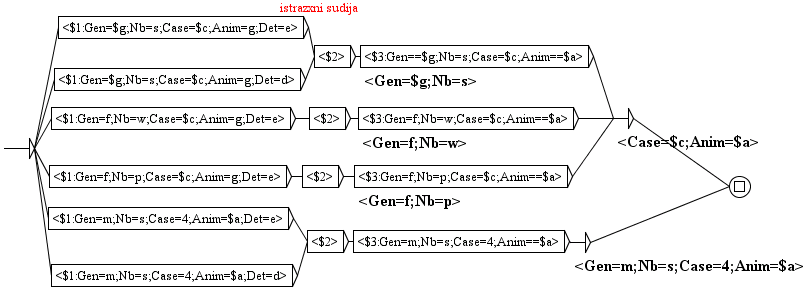
\includegraphics[width=15cm]{resources/img/NC'AXNF'SRB.png}
  \caption{Inflection graph \emph{NC\_AXNF} for Serbian MWUs}
  \label{fig:NC'AXNF'SRB}
\end{figure}

\begin{figure}[!htb]
  \centering
  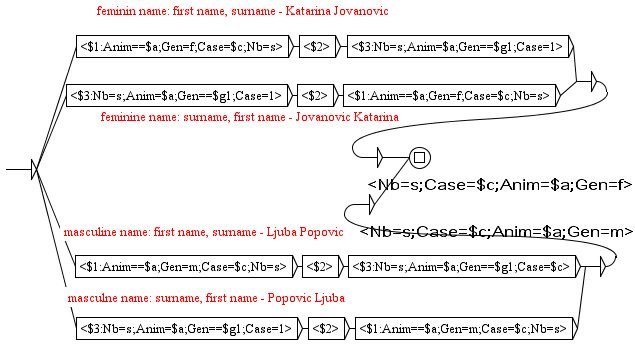
\includegraphics[width=15cm]{resources/img/NC'ImePrezime'SRB.png}
  \caption{Inflection graph \emph{NC\_ImePrezime} for Serbian MWUs}
  \label{fig:NC'ImePrezime'SRB}
\end{figure}

\begin{figure}[!htb]
  \centering
  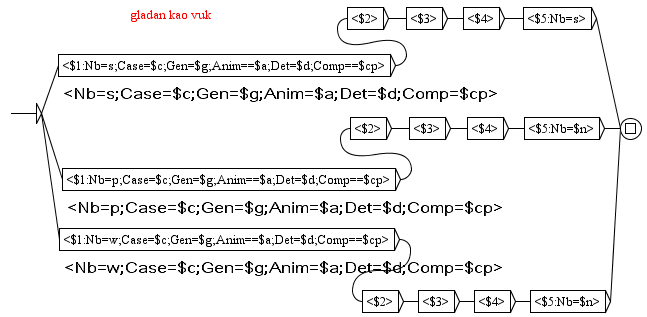
\includegraphics[width=15cm]{resources/img/AC'A3XN2'SRB.png}
  \caption{Inflection graph \emph{AC\_A3XN2} for Serbian MWUs}
  \label{fig:AC'A3XN2'SRB}
\end{figure}

%%%%%%%%%%%%%%%%%%%%%%%%%%%%%%%%%%%%%%%%%%%%%%%%%%%%%%%
